% Provenance (never printed): see sources/outline_sources.md (Year 3: primordial
% nucleosynthesis and stellar burning recalled from the physics books; the s and r
% processes; supernovae and neutron-star mergers; galactic chemical evolution; from the
% solar abundances to the composition of the Earth).
% Brief: sources/book5/BRIEFS.md, ch. 30. Curves from figdata/bachelor-3/
% solar_abundances.py (Asplund, Amarsi and Grevesse 2021, Table 2), neutron_capture.py
% (their Table B.1 isotopes, KADoNiS v0.3 cross sections, IAEA Live Chart half-lives) and
% chemical_evolution.py (closed box against the Geneva-Copenhagen survey of Casagrande et
% al. 2011, and a two-phase [alpha/Fe] model). Exercise and problem values in the Book 5
% scratch calculator calc/ch30.py.
\chapter{Waar de elementen vandaan komen}\label{ch:b3:origin-of-elements}

Het calcium van een kalksteenklif is grotendeels gemaakt in
massieve sterren die explodeerden voordat de Zon was geboren. Het ijzer van de
kern van de Aarde komt vooral uit een andere soort explosie, die van een
witte dwerg. Het platina van een ring hoort bij een abundantiepiek die is opgebouwd door
uitbarstingen van \omterm{def:b3:origin-of-elements:s-process}{neutronenvangsten} die seconden duren, in samensmeltingen van twee neutronensterren
of in een zeldzame soort supernova; welke van de twee het grootste deel ervan maakte, is
nog steeds omstreden.
Elk van deze gebeurtenissen heeft zijn sporen nagelaten in de samenstelling van de Zon,
die, op de paar elementen na die de planeten niet konden vasthouden, ook
de samenstelling van het Zonnestelsel is. Dit hoofdstuk leest dat verslag: het zet de \omterm{def:b3:origin-of-elements:abundance}{zonneabundanties} uiteen,
herinnert eraan hoe de lichte elementen zijn ontstaan, volgt de \omterm{def:b3:origin-of-elements:s-process}{neutronenvangsten} die de zware elementen opbouwden, zoekt
de plaatsen waar elk proces plaatsvindt, en modelleert hoe de samenstelling van een
sterrenstelsel verandert naarmate zijn sterren leven en sterven. Het eindigt waar de geologie van
de eerdere delen begint:
waarom de Aarde, gemaakt van hetzelfde materiaal als
de Zon, zo rijk is aan ijzer en zo arm aan vluchtige elementen.
% ledger: matteucci21:production, cowan21:rprocess, kobayashi20:origins, asplund21:fig1

\begin{recall}
Nucleosynthese van de oerknal, de fusie van waterstof en helium in sterren,
de bindingsenergie per nucleon en het maximum daarvan nabij ijzer, het dal van
de stabiliteit, bètaverval en halveringstijden, de werkzame doorsnede van een reactie,
hoofdreekssterren, rode reuzen, witte dwergen, neutronensterren en
supernova's staan in de natuurkundeboeken. De meteorietklassen, de
CI-chondrieten, de condensatietemperatuur, refractaire en vluchtige
elementen, de Goldschmidtklassen en de bulksilicaataarde worden
behandeld in Boek~4, in de hoofdstukken over de vorming van de planeten en over
de elementen in de Aarde. De structuur van de Melkweg, de dunne en
\omterm{def:b3:milky-way-galaxies:structure}{dikke schijf}, de halo en de \omterm{def:b3:milky-way-galaxies:populations}{sterpopulaties} staan in het vorige
hoofdstuk.
\end{recall}

\section{De zonneabundanties}\label{sec:b3:origin-of-elements:solar}

De Zon bevat meer dan \qty{99.85}{\percent} van de massa van het
Zonnestelsel, en haar buitenlagen hebben de samenstelling behouden, op een paar
lichte elementen en een langzame bezinking van de zware na, van het gas waaruit
de Zon en de planeten zijn gevormd. Men leest de samenstelling op twee manieren af:
uit de absorptielijnen van haar fotosfeer, en uit de CI-chondrieten,
de meteorieten waarvan de samenstelling, behalve voor de meest vluchtige
elementen, van alle bekende materialen het dichtst bij die van de Zon ligt.
% ledger: asplund21:fig1, asplund21:ci

\begin{definition}[Zonneabundantie; dex]\label{def:b3:origin-of-elements:abundance}
De \emph{zonneabundantie}\index{zonneabundantie} van een element $X$ is
het aantal van zijn atomen ten opzichte van die van waterstof in de Zon,
uitgedrukt op een logaritmische schaal waarop waterstof op $12$ wordt gesteld:
\[
\log\varepsilon(X) = 12 + \log_{10}\frac{N_X}{N_\mathrm{H}} .
\]
Een verschil van één eenheid in zo'n logaritme heet een
\emph{dex}\index{dex}: twee abundanties die $0.3$~dex van elkaar verschillen,
verschillen met een factor $10^{0.3} \approx 2$. Voor een ster wordt de abundantie ten opzichte van de
Zon met haakjes geschreven,
$[X/\mathrm{H}] = \log_{10}(N_X/N_\mathrm{H})_\star -
\log_{10}(N_X/N_\mathrm{H})_\odot$, en evenzo $[X/Y]$ voor elke twee
elementen.
\end{definition}

De onderstaande figuur toont de \omterm{def:b3:origin-of-elements:abundance}{zonneabundanties} van de recente compilatie
die alle 83 langlevende elementen opnieuw beoordeelt. IJzer, met
$\log\varepsilon = 7.46$, heeft één atoom op elke \num{34700} atomen
waterstof; helium heeft \num{0.0820} atomen per waterstofatoom. Enkele
kenmerken vallen op, en de rest van dit hoofdstuk verklaart ze.
% ledger: asplund21:abstract, asplund21:ci, data:b5-asplund21

\begin{omfigure}
\centering
\begin{tikzpicture}
\begin{axis}[width=0.95\linewidth, height=8.4cm, xmin=0, xmax=94,
  ymin=-1.8, ymax=12.8, xlabel={atoomgetal $Z$},
  ylabel={$\log\varepsilon(X)$ \;($\log\varepsilon(\mathrm{H}) = 12$)},
  tick label style={font=\scriptsize}, label style={font=\small},
  legend style={font=\scriptsize, at={(0.5,-0.17)}, anchor=north,
    legend columns=2, draw=none, cells={anchor=west},
    /tikz/every even column/.append style={column sep=1em}}]
\addplot[blue!70!black, mark=*, mark size=1.3pt, restrict x to domain=0:84]
  table[x=Z, y=logeps] {figdata/out/bachelor-3-solar_abundances-even.dat};
\addlegendentry{even $Z$}
\addplot[blue!70!black, mark=*, mark size=1.3pt, restrict x to domain=88:94, forget plot]
  table[x=Z, y=logeps] {figdata/out/bachelor-3-solar_abundances-even.dat};
\addplot[red!70!black, mark=o, mark size=1.4pt]
  table[x=Z, y=logeps] {figdata/out/bachelor-3-solar_abundances-odd.dat};
\addlegendentry{oneven $Z$}
\begin{scope}[font=\scriptsize]
\node[anchor=west] at (axis cs:2.2,12.2) {H};
\node[anchor=west] at (axis cs:3.0,10.9) {He};
\node[anchor=west] at (axis cs:5.6,1.0) {Li, Be, B};
\node[anchor=south] at (axis cs:8,8.95) {O};
\node[anchor=south] at (axis cs:6,8.6) {C};
\node[anchor=south, align=center] at (axis cs:26,7.75) {Fe\\[-1pt]piek};
\node[anchor=north] at (axis cs:21,2.95) {Sc};
\node[anchor=south, align=center] at (axis cs:38.5,3.05) {Sr--Zr\\[-1pt]($N = 50$)};
\node[anchor=south] at (axis cs:51.5,2.5) {Te, Xe (r)};
\node[anchor=south, align=center] at (axis cs:58.5,3.7) {Ba\\[-1pt]($N = 82$)};
\node[anchor=south] at (axis cs:76.5,1.95) {Pt (r)};
\node[anchor=south, align=center] at (axis cs:82.5,2.85) {Pb\\[-1pt]($N = 126$)};
\node[anchor=south] at (axis cs:89.6,0.15) {Th};
\node[anchor=north] at (axis cs:92,-0.7) {U};
\end{scope}
\end{axis}
\end{tikzpicture}
\par\smallskip{\small De \omterm{def:b3:origin-of-elements:abundance}{zonneabundanties} van de elementen in de Zon, op een
logaritmische schaal met waterstof op 12: fotosferische waarden, of die van de
CI-chondrieten voor de elementen die geen meetbare fotosferische
lijn hebben (Asplund, Amarsi en Grevesse, 2021). Even en oneven atoomgetallen
worden als twee lijnen getekend. Technetium ($Z = 43$) en promethium ($Z = 61$)
hebben geen langlevend isotoop, en dat geldt ook voor de elementen tussen bismut en
thorium.}\label{fig:b3:origin-of-elements:curve}
\end{omfigure}
% ledger: data:b5-asplund21, asplund21:fig1

\begin{enumerate}
\item Waterstof en helium vormen bijna alle atomen, duizend keer
  meer dan alle andere samen; beide ontstonden bij de Oerknal, en
  een deel van het helium sindsdien in sterren.
\item Lithium, beryllium en boor, net na helium, liggen ver onder
  koolstof: beryllium komt \num{12} miljoen keer minder voor.
\item De abundanties dalen steil van zuurstof naar de zware elementen,
  met pieken rond zuurstof, rond ijzer, rond barium en rond lood, en
  kleinere pieken die de figuur aangeeft.
\item Elementen met een even atoomgetal komen meer voor dan hun oneven
  buren: scandium, tussen calcium en titanium, is ongeveer \num{1400}
  keer zeldzamer dan calcium en \num{68} keer zeldzamer dan titanium. Dit
  is het \emph{even-oneven-effect}.
\item Voorbij de ijzerpiek vlakt de curve af: van ijzer naar goud daalt
  de abundantie met een factor \num{3.5e6}, maar van goud naar lood
  stijgt ze weer, met een factor elf.
\end{enumerate}
% ledger: asplund21:fig1, data:b5-asplund21

Op massabasis is de huidige fotosfeer $X = 0.7438$ waterstof,
$Y = 0.2423$ helium en $Z = 0.0139$ van al het overige. Gecorrigeerd voor
de zware elementen die sinds de vorming van de Zon onder de fotosfeer zijn
bezonken, zijn de protosolaire waarden, die van het gas waaruit de Zon
ontstond, $X = 0.7121$, $Y = 0.2725$ en $Z = 0.0154$.
% ledger: asplund21:xyz

\begin{definition}[Metalliciteit]\label{def:b3:origin-of-elements:metallicity}
De \emph{metalliciteit}\index{metalliciteit} van een ster of van een gas is
het gehalte aan elementen zwaarder dan helium, in de astronomie metalen
genoemd, ongeacht hun chemie: als massafractie $Z$, of, zoals het meestal
wordt gemeten, als de ijzerabundantie ten opzichte van de Zon, $[\mathrm{Fe/H}]$.
Een ster met $[\mathrm{Fe/H}] = -1$ heeft per waterstofatoom een tiende
van het ijzer van de Zon.
\end{definition}

De twee bronnen van de \omterm{def:b3:origin-of-elements:abundance}{zonneabundanties} komen opvallend goed overeen. De
figuur hieronder vergelijkt ze element voor element. Voor 58 elementen,
die niet te vluchtig zijn voor de meteorieten en niet in de Zon zijn
vernietigd, is het gewogen gemiddelde verschil tussen de fotosferische en
de CI-abundantie $\num[separate-uncertainty=true]{0.000 \pm 0.007}$~\omterm{def:b3:origin-of-elements:abundance}{dex}.
Twee groepen vallen buiten de lijn. De meteorieten bevatten veel minder
waterstof, helium, koolstof, stikstof, zuurstof en edelgassen dan de Zon:
deze elementen bleven in het gas toen de vaste stoffen condenseerden. De
Zon bevat \num{200} keer minder lithium dan de meteorieten: ze heeft
\qty{99.5}{\percent} van haar lithium door kernverbranding vernietigd.
% ledger: asplund21:ci, data:b5-asplund21

\begin{omfigure}
\centering
\begin{tikzpicture}
\begin{axis}[width=0.66\linewidth, height=0.66\linewidth, xmin=-3, xmax=12.8,
  ymin=-1, ymax=12.8, xlabel={$\log\varepsilon$ in de CI-chondrieten},
  ylabel={$\log\varepsilon$ in de fotosfeer},
  tick label style={font=\scriptsize}, label style={font=\small},
  scatter/classes={0={mark=*, mark size=1.3pt, black!70},
    1={mark=square*, mark size=1.5pt, red!70!black},
    2={mark=triangle*, mark size=2pt, blue!70!black}}]
\addplot[black!40, dashed, domain=-1:12.8, samples=2] {x};
\addplot[scatter, only marks, scatter src=explicit symbolic]
  table[x=ci, y=phot, meta=group] {figdata/out/bachelor-3-solar_abundances-compare.dat};
\begin{scope}[font=\scriptsize, red!60!black]
\node[anchor=east] at (axis cs:8.12,12.0) {H};
\node[anchor=west] at (axis cs:1.45,10.914) {He};
\node[anchor=east] at (axis cs:7.25,8.55) {C};
\node[anchor=east] at (axis cs:6.1,7.83) {N};
\node[anchor=west] at (axis cs:8.5,8.45) {O};
\node[anchor=west] at (axis cs:-0.97,8.06) {Ne};
\node[anchor=west] at (axis cs:-0.35,6.38) {Ar};
\node[anchor=west] at (axis cs:-2.12,3.12) {Kr};
\node[anchor=west] at (axis cs:-1.8,2.22) {Xe};
\end{scope}
\node[font=\scriptsize, blue!60!black, anchor=west] at (axis cs:3.4,0.96) {Li};
\end{axis}
\end{tikzpicture}
\par\smallskip{\small De Zon tegenover de CI-chondrieten: elk punt is één
element met beide waarden (Asplund, Amarsi en Grevesse, 2021; de
meteoritische schaal is zo vastgelegd dat silicium overeenkomt). De
stippellijn is gelijkheid. Zwarte stippen: de 58 elementen die
overeenkomen. Vierkanten: waterstof, helium, koolstof, stikstof, zuurstof
en de edelgassen, die de meteorieten niet hebben behouden. Driehoek:
lithium, in de Zon vernietigd.}\label{fig:b3:origin-of-elements:sun-ci}
\end{omfigure}
% ledger: data:b5-asplund21, asplund21:ci

De overeenstemming is een feit van groot gewicht voor de geologie. Ze
betekent dat de meteorieten, die in het laboratorium kunnen worden
geanalyseerd, de samenstelling van het Zonnestelsel geven voor alle
elementen behalve de meest vluchtige; en dat de Zon, waarvan de fotosfeer
waterstof, koolstof, stikstof en zuurstof geeft, vult de rest aan. Het
tweede jaar bouwde op dat fundament de samenstelling van de bulk-Aarde op.
% ledger: asplund21:ci

\section{De lichte elementen en de sterren}\label{sec:b3:origin-of-elements:stars}

De natuurkundeboeken beschrijven de nucleosynthese van de Oerknal: in de
eerste drie minuten, terwijl het heelal afkoelde, verbonden protonen en
neutronen zich tot deuterium, helium-3, helium-4 en een spoor lithium-7, en
tot niets zwaarder. De waargenomen primordiale abundanties zijn een heliummassafractie
$Y_\mathrm{p} = \num[separate-uncertainty=true]{0.245 \pm 0.003}$, een
deuterium-tot-waterstofverhouding van \num{2.5e-5} en een
lithium-tot-waterstofverhouding van \num{1.45e-10}, de laatste gemeten in oude
metaalarme sterren van de galactische halo. Alle andere elementen, en het
overschot aan helium in de Zon, $0.2725 - 0.245 \approx 0.028$, zijn in sterren gevormd.
% ledger: pdg25:bbn, asplund21:xyz

De sterren uit de natuurkundeboeken verbranden waterstof tot helium op de
hoofdreeks, daarna helium tot koolstof en zuurstof als rode reuzen; de
zwaarste gaan verder, in schillen rond hun kern, tot neon, magnesium,
silicium en tenslotte ijzer. Bij ijzer houdt de fusie op, omdat de
bindingsenergie per nucleon daar het grootst is: het opbouwen van zwaardere
kernen door fusie kost energie in plaats van dat het er oplevert. Voorbij de
ijzerpiek worden de elementen op een andere manier gevormd, door het
vangen van neutronen, het onderwerp van de volgende paragraaf. Lithium,
beryllium en boor zijn broos: ze worden vernietigd bij de temperaturen
in het inwendige van sterren, waarom de Zon bijna al haar lithium heeft
verbrand en waarom de drie elementen een dal vormen in de abundantiecurve.

\begin{definition}[Alfa-element]\label{def:b3:origin-of-elements:alpha}
Een \emph{alfa-element}\index{alfa-element} is een van de elementen met een even $Z$
zuurstof, neon, magnesium, silicium, zwavel en calcium, waarvan de
meest voorkomende isotopen ($^{16}\mathrm{O}$, $^{20}\mathrm{Ne}$,
$^{24}\mathrm{Mg}$, $^{28}\mathrm{Si}$, $^{32}\mathrm{S}$,
$^{40}\mathrm{Ca}$) massagetallen hebben die een veelvoud van vier zijn, en
die vooral in massieve sterren worden gevormd en via hun explosie als
kernineenstortingssupernova's aan het gas worden teruggegeven.
\end{definition}
% ledger: matteucci21:production, data:b5-asplund21

De pieken van zuurstof en van de \omterm{def:b3:origin-of-elements:alpha}{alfa-elementen}, en het oneven-even-effect,
zijn de kenmerken van deze brandfasen: heliumkernen worden gemakkelijker in de even kernen
ingebouwd dan in de oneven, en kernen
met een even aantal protonen zijn steviger gebonden. Wat een ster aan het gas teruggeeft
hangt af van zijn massa.

\begin{definition}[Stellaire opbrengst]\label{def:b3:origin-of-elements:yield}
De \emph{stellaire opbrengst}\index{stellaire opbrengst} van een element van een ster
met een gegeven beginmassa is de massa van dat element die de ster
nieuw heeft gevormd en teruggeeft aan het interstellaire gas, in winden en in zijn
uiteindelijke explosie, als fractie van de massa van de ster.
\end{definition}
% ledger: matteucci21:yield

Sterren van minder dan \qty{0.8}{M_\odot} leven langer dan de ouderdom van het
heelal en geven niets terug. Sterren van \num{0.8} tot \qty{8}{M_\odot}
geven helium, stikstof, koolstof en de zware elementen van het \omterm{def:b3:origin-of-elements:s-process}{s-proces}
(barium, yttrium, strontium) via hun winden terug, en eindigen als koolstof-zuurstof
witte dwergen. Sterren van meer dan \num{8} tot \qty{10}{M_\odot} maken
vooral de \omterm{def:b3:origin-of-elements:alpha}{alfa-elementen} en wat ijzer, en exploderen als
kernineenstortingssupernova's. Een witte dwerg in een nauwe dubbelster kan exploderen als Type~Ia
supernova, en zulke explosies leveren het grootste deel van het ijzer.
% ledger: matteucci21:production

\begin{omfigure}
\centering
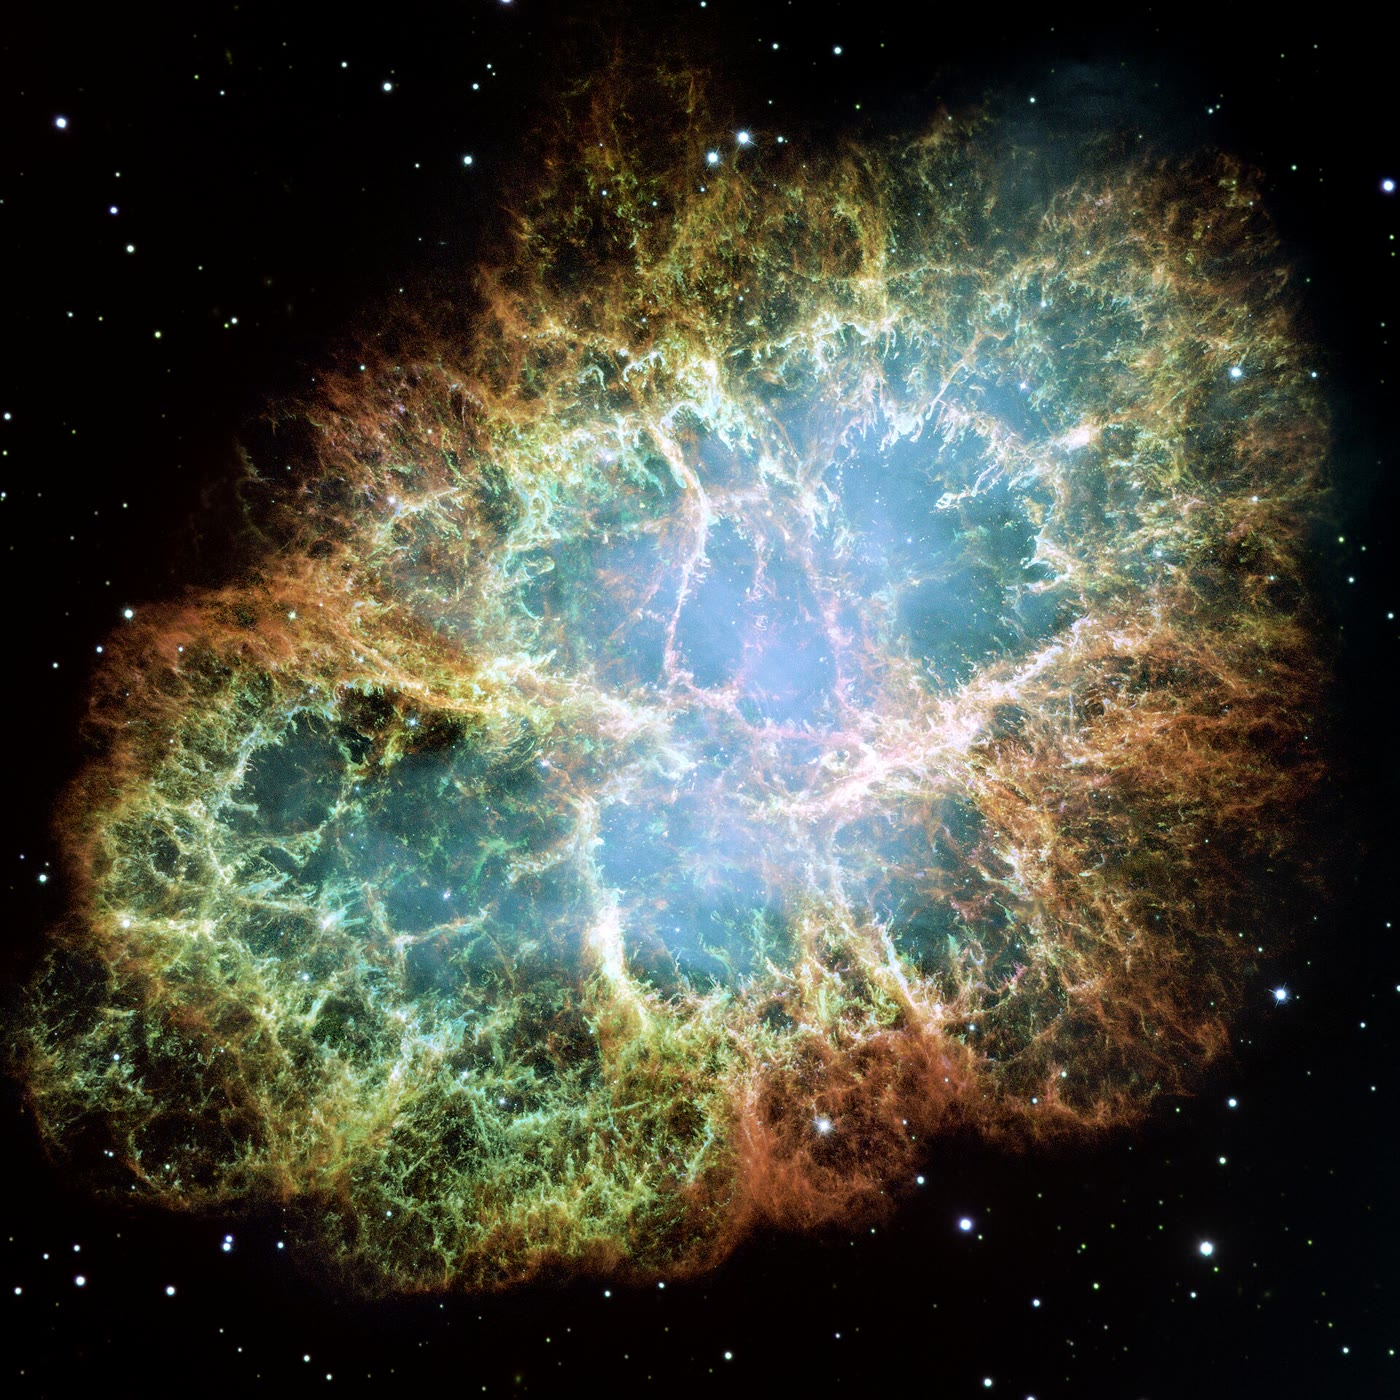
\includegraphics[width=0.5\linewidth]{images/book5/b3-crab-nebula.jpg}
\par\smallskip{\small De Krabnevel, een mozaïek van 24 Hubble Space
Telescope-opnamen: de uitdijende overblijfselen van een ster waarvan de explosie
Japanse en Chinese astronomen registreerden in 1054. De oranje filamenten
zijn de gerafelde buitenlagen van de ster, vooral waterstof; de blauwachtige
gloed binnenin komt van elektronen die in spiralen rond de magnetische
veldlijnen van de neutronenster in het midden, die dertig keer per
seconde ronddraait. Het gas van de filamenten, dat meedraagt wat de ster heeft gemaakt, mengt zich
in het interstellaire medium. NASA, ESA, J.~Hester en A.~Loll, publiek
domein.}\label{fig:b3:origin-of-elements:crab}
\end{omfigure}
% ledger: photo:b3-crab-nebula

\section{Neutronenvangsten}\label{sec:b3:origin-of-elements:neutrons}

Een neutron heeft geen elektrische lading en wordt niet afgestoten door een kern: zelfs
een langzaam neutron dringt er binnen, en de kern, één massa-eenheid zwaarder, geeft
de bindingsenergie af als gammastraling. Herhaalde vangsten maken zwaardere
isotopen van hetzelfde element, totdat er één onstabiel is; die vervalt dan,
meestal door bètaminusverval in het volgende element, dat op zijn beurt
vangt. Welke kernen er ontstaan, hangt af van één vergelijking: de tijd tussen
twee vangsten, afgezet tegen de halveringstijd van de onstabiele kernen die
onderweg worden tegengekomen.

\begin{definition}[Neutronenvangst; s-proces; r-proces]\label{def:b3:origin-of-elements:s-process}
\emph{Neutronenvangst}\index{neutronenvangst} is de opname van een
vrij neutron door een kern, $(Z, A) + \mathrm{n} \to (Z, A+1) + \gamma$.
In het \emph{s-proces}\index{s-proces} (langzaam) zijn de vangsten
trager dan de meeste bètavervallen: de tijd tussen twee vangsten aan één
kern is honderden tot duizenden jaren, zodat een onstabiele kern
bijna altijd vervalt voordat hij kan vangen, en de keten van vangsten en vervallen
volgt het stabiliteitsdal. In het
\emph{r-proces}\index{r-proces} (snel), is de neutronendichtheid
zo hoog dat de vangsten veel sneller verlopen dan het verval: de kernen worden
gedreven naar zeer neutronenrijke isotopen, ver van de stabiliteit, in enkele
seconden, en vervallen terug naar de stabiliteit zodra de neutronen op zijn.
\end{definition}
% ledger: cowan21:timescales, cowan21:rprocess, kaeppeler11:overview

De twee processen bereiken verschillende kernen, en de nuclidenkaart
laat zien welke. De figuur hieronder toont een strook daarvan, van cadmium tot
barium. Het \omterm{def:b3:origin-of-elements:s-process}{s-proces} klimt erlangs het stabiliteitsdal: langs een
rij van een element zolang de isotopen stabiel zijn, en dan één rij omhoog door een
bètaverval. Het \omterm{def:b3:origin-of-elements:s-process}{r-proces} komt van de neutronenrijke kant, rechtsonder:
elke zeer neutronenrijke kern vervalt door opeenvolgende
bètaminusvervallen langs zijn isobaar, met behoud van zijn massagetal, en stopt
bij de eerste stabiele kern die hij tegenkomt. Een stabiele kern die een stabiele isobaar
met een lagere $Z$ heeft, is \emph{afgeschermd} tegen het \omterm{def:b3:origin-of-elements:s-process}{r-proces}: $^{122}\mathrm{Te}$
ligt achter $^{122}\mathrm{Sn}$, $^{123}\mathrm{Te}$ achter
$^{123}\mathrm{Sb}$, $^{124}\mathrm{Te}$ achter $^{124}\mathrm{Sn}$.
Die drie kunnen alleen door het \omterm{def:b3:origin-of-elements:s-process}{s-proces} worden gevormd: ze zijn
\emph{alleen-s}. Omgekeerd liggen $^{128}\mathrm{Te}$ en $^{130}\mathrm{Te}$
voorbij het s-pad, waardoor telluur alleen overblijft bij $^{127}\mathrm{Te}$,
waarvan de halveringstijd \qty{9.35}{h} is: die zijn alleen-r.
% ledger: kaeppeler11:overview, data:b5-iaea-gs, data:b5-sigman

\begin{omfigure}
\centering
\begin{tikzpicture}
\begin{axis}[x=0.62cm, y=0.7cm, xmin=61.4, xmax=84.6, ymin=47.4, ymax=56.6,
  xlabel={neutrongetal $N$}, ylabel={},
  xtick={62,64,...,84}, ytick={48,...,56},
  yticklabels={Cd 48, In 49, Sn 50, Sb 51, Te 52, I 53, Xe 54, Cs 55, Ba 56},
  tick label style={font=\scriptsize}, label style={font=\small},
  axis line style={black!40}, clip=false,
  scatter/classes={0={mark=square*, mark size=6.5pt, blue!45},
    1={mark=square*, mark size=6.5pt, black!18},
    2={mark=square*, mark size=6.5pt, red!40},
    3={mark=square*, mark size=6.5pt, orange!45}}]
\addplot[only marks, mark=square, mark size=6.5pt, black!45, thin,
  restrict x to domain=61:85]
  table[x=N, y=Z] {figdata/out/bachelor-3-neutron_capture-unstable.dat};
\addplot[scatter, only marks, scatter src=explicit symbolic,
  restrict x to domain=61:85]
  table[x=N, y=Z, meta=cls] {figdata/out/bachelor-3-neutron_capture-chart.dat};
\addplot[only marks, mark=none, nodes near coords={\massnum},
  restrict x to domain=61:85,
  visualization depends on={value \thisrow{A} \as \massnum},
  nodes near coords align={center}, every node near coord/.append style={font=\tiny}]
  table[x=N, y=Z] {figdata/out/bachelor-3-neutron_capture-chart.dat};
\addplot[only marks, mark=none, nodes near coords={\massnum}, restrict x to domain=61:85,
  visualization depends on={value \thisrow{A} \as \massnum},
  nodes near coords align={center}, every node near coord/.append style={font=\tiny, black!55}]
  table[x=N, y=Z] {figdata/out/bachelor-3-neutron_capture-unstable.dat};
\addplot[quiver={u=0.48*\thisrow{dN}, v=0.48*\thisrow{dZ}}, -{Stealth[length=3pt]},
  blue!60!black, semithick, restrict x to domain=61:85]
  table[x expr=\thisrow{N0}+0.26*\thisrow{dN}, y expr=\thisrow{Z0}+0.26*\thisrow{dZ}]
  {figdata/out/bachelor-3-neutron_capture-path.dat};
\begin{scope}[red!70!black, dashed, -{Stealth[length=4pt]}, thick]
\draw (axis cs:79.1,48.9) -- (axis cs:76.4,51.6);
\draw (axis cs:81.1,48.9) -- (axis cs:78.4,51.6);
\draw (axis cs:83.1,50.9) -- (axis cs:80.4,53.6);
\end{scope}
\node[font=\scriptsize, red!70!black, anchor=south east, align=right] at (axis cs:84.5,47.5)
  {r-proces-vervallen\\[-1pt]langs isobaren};
\end{axis}
\end{tikzpicture}
\par\smallskip{\small Een strook van de nuclidenkaart, van cadmium
tot barium, neutrongetallen 62 tot 84. Gekleurde vierkanten zijn de in de natuur voorkomende kernen, voorzien
van hun massagetal: blauw, alleen-s; grijs, door beide processen gevormd; rood,
alleen-r; oranje, \omterm{def:b3:origin-of-elements:p-process}{p-kernen}, door geen van beide bereikt. Open vierkanten zijn de
onstabiele kernen die het \omterm{def:b3:origin-of-elements:s-process}{s-proces} doorloopt. Blauwe pijlen: het s-pad,
vangsten naar rechts, bètavervallen diagonaal omhoog en naar links (bij
$^{134}\mathrm{Cs}$ en $^{135}\mathrm{Cs}$ splitst het pad). Gestreepte rode
pijlen: drie van de vervalketens van het \omterm{def:b3:origin-of-elements:s-process}{r-proces}, eindigend op
$^{128}\mathrm{Te}$, $^{130}\mathrm{Te}$ en $^{134}\mathrm{Xe}$. De
klassen zijn berekend uit de in de natuur gevonden isotopen (Asplund,
Amarsi en Grevesse, 2021) en de halveringstijden en vervalwijzen van de
IAEA-nuclidenkaart.}\label{fig:b3:origin-of-elements:chart}
\end{omfigure}
% ledger: data:b5-sigman, data:b5-iaea-gs, data:b5-asplund21, kaeppeler11:branchings

Een derde groep, de oranje vierkanten, wordt door geen van beide processen bereikt: de
protonrijke isotopen zoals $^{112}\mathrm{Sn}$, $^{120}\mathrm{Te}$
of $^{124}\mathrm{Xe}$.

\begin{definition}[p-kernen]\label{def:b3:origin-of-elements:p-process}
De \emph{p-kernen}\index{p-kernen} zijn de stabiele isotopen aan de
protonrijke kant van het stabiliteitsdal, voorbij de ijzerpiek, die
noch het s- noch het \omterm{def:b3:origin-of-elements:s-process}{r-proces} kan maken: ze zijn afgeschermd tegen het \omterm{def:b3:origin-of-elements:s-process}{r-proces}
door een stabiele isobaar met lager $Z$ en liggen buiten het s-pad. Ze
worden toegeschreven aan een afzonderlijk p-proces, waarschijnlijk in supernova-explosies, en
op enkele uitzonderingen na is hun overvloed veel kleiner dan die van de
naburige s- en r-isotopen.
\end{definition}
% ledger: kaeppeler11:overview

De regel die de kaart leest, toegepast op alle 287 nuclides van de
protosolaire tabel voorbij zink, levert 30 alleen-s-nuclides, 29 alleen-r-nuclides
en 36 \omterm{def:b3:origin-of-elements:p-process}{p-kernen} op. Eén van deze \omterm{def:b3:origin-of-elements:p-process}{p-kernen}, $^{176}\mathrm{Hf}$, wordt in feite
door het \omterm{def:b3:origin-of-elements:s-process}{s-proces} bereikt via een langlevende aangeslagen toestand van
$^{176}\mathrm{Lu}$ die de eenvoudige regel negeert; de overige 35 zijn de \omterm{def:b3:origin-of-elements:p-process}{p-kernen}
uit de literatuur.
% ledger: data:b5-sigman, kaeppeler11:branchings

Het \omterm{def:b3:origin-of-elements:s-process}{s-proces} kan kwantitatief worden gevolgd, omdat zijn nuclides dicht bij de stabiliteit liggen en
hun vangstdoorsneden gemeten kunnen worden. In een stellair plasma
bij temperatuur $T$ zijn de neutronen thermisch, en wat telt is
de doorsnede gemiddeld over hun Maxwell--Boltzmann-
verdeling, $\langle\sigma\rangle$, opgegeven voor een thermische energie
$kT = \qty{30}{keV}$.
% ledger: kaeppeler11:classical

\begin{proposition}[De $\sigma N$-relatie]\label{prop:b3:origin-of-elements:sigma-n}
\index{sigma N-relatie@$\sigma N$-relatie}
Op een traject van het s-pad waar elke kern stabiel is en de neutronendichtheid
$n_\mathrm{n}$ en temperatuur constant zijn, zij $N_A$ de
overvloed van de kern met massagetal $A$ en $\langle\sigma\rangle_A$
haar gemiddelde doorsnede. Als de neutronenstroom een stationaire
toestand heeft bereikt, dan geldt
\[
\langle\sigma\rangle_{A-1} N_{A-1} = \langle\sigma\rangle_A N_A ,
\]
zodat het product $\sigma N$ voor elke kern van het
traject hetzelfde is.
\end{proposition}

\begin{proof}
Een kern met massa $A$ vangt neutronen op met de snelheid
$\lambda_A = n_\mathrm{n}\langle\sigma\rangle_A v_T$ per kern, waarbij
$v_T$ de gemiddelde thermische snelheid van de neutronen is. Ze wordt gevormd door vangsten op
$A - 1$ en vernietigd door vangsten op zichzelf, dus
$\mathrm{d}N_A/\mathrm{d}t = n_\mathrm{n} v_T\,(\langle\sigma\rangle_{A-1}
N_{A-1} - \langle\sigma\rangle_A N_A)$. In een stationaire toestand verdwijnt de
afgeleide, en dat is de relatie. Een kern met een grote doorsnede wordt
snel doorgegeven en blijft zeldzaam; een kern met een kleine doorsnede hoopt
zich op.
\end{proof}
% ledger: kaeppeler11:classical

De drie alleen-s-isotopen van tellurium toetsen dit. Hun protosolaire
overvloed bedraagt \num{0.1067}, \num{0.0373} en \num{0.1984} atomen per
miljoen siliciumatomen, en hun doorsneden \num{295}, \num{832} en
\qty{155}{mb}: de producten zijn \num{31.5}, \num{31.0} en
\qty{30.8}{mb}, gelijk binnen drie procent, hoewel de overvloeden
een factor vijf verschillen. Over een neutronenmagisch getal breekt de relatie:
kernen met $N = 50$, $82$ of $126$ zijn zo sterk gebonden dat
ze slecht vangen, $\langle\sigma\rangle = \qty{4.0}{mb}$ voor
$^{138}\mathrm{Ba}$ tegenover \qty{61.2}{mb} voor $^{136}\mathrm{Ba}$, en
ze werken als flessenhalzen. De figuur hieronder toont het product voor alle
alleen-s-nuclides: vlakke plateaus gescheiden door sprongen nabij $A = 88$, $140$
en $208$.
% ledger: data:b5-sigman, data:b5-kadonis, kaeppeler11:classical

\begin{omfigure}
\centering
\begin{tikzpicture}
\begin{axis}[width=0.95\linewidth, height=7.4cm, xmin=60, xmax=212,
  ymode=log, ymin=1, ymax=5000, xlabel={massagetal $A$},
  ylabel={$\langle\sigma\rangle N$ (mb, per $10^6$ Si-atomen)},
  tick label style={font=\scriptsize}, label style={font=\small},
  legend style={font=\scriptsize, at={(0.5,-0.17)}, anchor=north,
    legend columns=2, draw=none, cells={anchor=west},
    /tikz/every even column/.append style={column sep=1em}}]
\draw[black!35, dotted, thick] (axis cs:88,1) -- (axis cs:88,5000);
\draw[black!35, dotted, thick] (axis cs:139,1) -- (axis cs:139,5000);
\draw[black!35, dotted, thick] (axis cs:208,1) -- (axis cs:208,5000);
\addplot[blue!70!black, thick, const plot]
  table[x=A, y=sigN_model] {figdata/out/bachelor-3-neutron_capture-fitted.dat};
\addlegendentry{klassiek model gefit voor $A > 90$}
\addplot[only marks, mark=*, mark size=1.7pt, red!70!black]
  table[x=A, y=sigN] {figdata/out/bachelor-3-neutron_capture-sigman.dat};
\addlegendentry{alleen-s-nuclides}
\begin{scope}[font=\scriptsize]
\node[anchor=south west] at (axis cs:88.5,1.1) {$N = 50$};
\node[anchor=south west] at (axis cs:139.5,1.1) {$N = 82$};
\node[anchor=south east] at (axis cs:207.5,1.1) {$N = 126$};
\node[anchor=south] at (axis cs:123,38) {Te};
\node[anchor=south] at (axis cs:135,33) {Ba};
\node[anchor=north] at (axis cs:149,6.6) {Sm};
\node[anchor=west] at (axis cs:177,1.79) {Lu};
\node[anchor=west] at (axis cs:71,2326) {Ge};
\node[anchor=west] at (axis cs:83,428) {Kr};
\end{scope}
\end{axis}
\end{tikzpicture}
\par\smallskip{\small Het product van de neutronenvangstdoorsnede
bij \qty{30}{keV} (KADoNiS) en de protosolaire overvloed (Asplund,
Amarsi en Grevesse, 2021) voor de 30 alleen-s-nuclides. Tussen de magische
neutronengetallen (stippellijnen) is het bijna constant; bij elk daarvan wordt de stroom
gesmoord en daalt het product. De lijn is het klassieke model
van het \omterm{def:b3:origin-of-elements:s-process}{s-proces}, hier gefit op de kernen zwaarder dan $A = 90$. De
lichtere hebben een tweede, zwakkere component nodig, gemaakt in massieve
sterren.}\label{fig:b3:origin-of-elements:sigma-n}
\end{omfigure}
% ledger: data:b5-sigman, data:b5-kadonis, data:b5-asplund21, kaeppeler11:classical

De lijn in de figuur is het klassieke model van het \omterm{def:b3:origin-of-elements:s-process}{s-proces}: een kleine
fractie $G$ van het ijzer-56 wordt aan neutronen blootgesteld, waarbij de
blootstellingen exponentieel verdeeld zijn rond een gemiddelde $\tau_0$, en de
stroom wordt kern voor kern gevolgd met de gemeten werkzame doorsneden. De fit
op 22 uitsluitend-s-kernen zwaarder dan $A = 90$ (met weglating van $^{176}\mathrm{Lu}$,
dat vervalt, en $^{187}\mathrm{Os}$, dat gevoed wordt door het verval van
$^{187}\mathrm{Re}$) levert $\tau_0 = \qty{0.31}{mb^{-1}}$ en
$G = \qty{0.054}{\percent}$ van het zonne-ijzer-56, dicht bij de
\qty{0.04}{\percent} uit de gedetailleerde analyses, waarin elke zaadkern
gemiddeld ongeveer vijftien neutronen opvangt. De lichtste uitsluitend-s-kernen,
germanium-70 en seleen-76, liggen ver boven de lijn: zij hebben een
tweede, zwakke component nodig, gemaakt in zware sterren.
% ledger: data:b5-sigman, kaeppeler11:classical

Waar een onstabiele kern op het pad ongeveer even lang leeft als de tijd
tussen twee invangsten, splitst de stroom zich: een deel vervalt, een deel
vangt in. Zulke \emph{vertakkingen} treden op bij $^{79}\mathrm{Se}$, $^{85}\mathrm{Kr}$,
$^{134}\mathrm{Cs}$, $^{147}\mathrm{Pm}$ en $^{151}\mathrm{Sm}$, onder andere.
Een vertakking laat een deel van de stroom een kern omzeilen: van de twee
uitsluitend-s-isotopen van samarium ontvangt $^{150}\mathrm{Sm}$ de volledige
stroom, en $^{148}\mathrm{Sm}$ alleen het deel dat langs de vertakking bij
massa 147 ging, en de verhouding van hun $\sigma N$, \num{0.87}, meet dat
aandeel. Omdat het aandeel afhangt van de neutronendichtheid en de
temperatuur, zijn de vertakkingen thermometers en densimeters van de sterren
waar het \omterm{def:b3:origin-of-elements:s-process}{s-proces} plaatsvond.
% ledger: kaeppeler11:branchings, kaeppeler11:pairs, data:b5-sigman

\begin{inthelab}[Een invangstdoorsnede meten]
Om de gemiddelde doorsneden te meten die het \omterm{def:b3:origin-of-elements:s-process}{s-proces} nodig heeft, reproduceren
natuurkundigen bij een versneller een stellair neutronenspectrum. Protonen die
op een lithiumdoelwit botsen, maken neutronen via de reactie
$^{7}\mathrm{Li}(\mathrm{p},\mathrm{n})^{7}\mathrm{Be}$, waarvan het spectrum
een thermisch spectrum nabootst bij $kT = \qty{25}{keV}$, dicht bij de
\qty{23}{keV} van de heliumschilflitsen van een rode reus. Het monster zit
direct tegen het doelwit, in de sterkste flux, en na de bestraling worden de
gammastralen van de nieuw gevormde radioactieve kernen geteld: deze
activeringsmethode werkt met monsters van minder dan een microgram. Waar het
product stabiel is, worden de neutronen in pulsen verzonden en over een
vliegbaan gemeten om hun energie te bepalen, en een bol van
bariumfluoridekristallen rond het monster registreert de gammastralingscascade
van elke invangst.
\end{inthelab}
% ledger: kaeppeler11:lab

\begin{history}[Technetium in rode reuzen]
In 1952 vond P.~W.~Merrill de lijnen van technetium in de spectra van
rode reuzen van spectraaltype S. Technetium heeft geen stabiele isotoop; de
isotoop die door het \omterm{def:b3:origin-of-elements:s-process}{s-proces} gemaakt wordt, $^{99}\mathrm{Tc}$, heeft een
halveringstijd van \num{211000} jaar, veel korter dan de levensduur die deze
sterren hadden. Het technetium moest binnen de sterren en recent gevormd zijn.
Het was het eerste directe bewijs dat sterren elementen maken. In
1957 formuleerden E.~M. en G.~R.~Burbidge, W.~A.~Fowler en F.~Hoyle, en
onafhankelijk A.~G.~W.~Cameron, het klassieke model van het
\omterm{def:b3:origin-of-elements:s-process}{s-proces}.
\end{history}
% ledger: kaeppeler11:overview, data:b5-iaea-gs

Het \omterm{def:b3:origin-of-elements:s-process}{r-proces} laat zijn eigen pieken achter. Het pad loopt dicht langs de
neutronendruiplijn, de grens waarachter een kern geen extra neutron meer kan
vasthouden, en de stroom wacht bij de kernen met gesloten neutronenschillen,
$N = 50$, $82$ en $126$, totdat ze bètaverval ondergaan. Deze wachtpunten
hopen materiaal op; na de laatste vervallen tot stabiliteit liggen de hopen
bij massagetallen die enkele eenheden lager zijn dan de s-procespieken bij
dezelfde magische getallen, die uit stabiele kernen bestaan: nabij $A = 130$
(telluur en xenon) en $A = 195$ (platina), tegenover $A = 138$ en $208$ voor de
s-pieken van barium en lood. De abundantiecurve toont beide reeksen pieken
naast elkaar. Het \omterm{def:b3:origin-of-elements:s-process}{r-proces} maakt ongeveer de helft van de zware elementen, het
\omterm{def:b3:origin-of-elements:s-process}{s-proces} de andere helft.
% ledger: cowan21:rprocess, kaeppeler11:overview, kaeppeler11:classical

\section{Waar de processen plaatsvinden}\label{sec:b3:origin-of-elements:sites}

Het belangrijkste \omterm{def:b3:origin-of-elements:s-process}{s-proces} vindt plaats in rode reuzen tot ongeveer drie zonsmassa's,
tegen het eind van hun leven, als sterren op de asymptotische reuzentak. Tussen de flitsen
van heliumverbranding in een schil rond hun kernen vormt zich een dunne laag rijk
aan koolstof-13; bij ongeveer \qty{9e7}{K} geeft de reactie
$^{13}\mathrm{C}(\alpha,\mathrm{n})^{16}\mathrm{O}$ gedurende enkele tienduizend jaar
neutronen vrij, bij dichtheden van $10^6$ tot
\num{e8}\text{ neutronen}\,\unit{cm^{-3}}. Tijdens de flitsen zelf, boven
\qty{2.5e8}{K}, levert $^{22}\mathrm{Ne}(\alpha,\mathrm{n})^{25}\mathrm{Mg}$
een uitbarsting van enkele jaren bij maximaal \qty{e10}{cm^{-3}}. De producten
worden naar het oppervlak meegevoerd, waar technetium waargenomen wordt, en
weggeblazen door de sterrenwind. Het zwakke \omterm{def:b3:origin-of-elements:s-process}{s-proces}, dat de uitsluitend-s-kernen
lichter dan $A = 90$ maakt, vindt plaats in zware sterren tijdens hun heliumverbranding
en koolstofverbranding.
% ledger: kaeppeler11:sources, kaeppeler11:overview

Kernval-supernova's, het einde van sterren boven acht tot tien zonsmassa's,
leveren de \omterm{def:b3:origin-of-elements:alpha}{alfa-elementen} en een deel van het ijzer kort na de geboorte van de sterren,
omdat zware sterren korte levens hebben. Type~Ia-supernova's, witte dwergen die in
dubbelsterren ontploffen, leveren het grootste deel van het ijzer, maar pas na een
vertraging: de witte dwerg moet eerst ontstaan uit een ster van minder dan acht
zonsmassa's, en dan ofwel materie van een metgezel verzamelen tot hij de
Chandrasekhar-massa bereikt, ongeveer
\qty{1.44}{M_\odot}, ofwel samensmelten met een tweede witte dwerg. Het \omterm{def:b3:origin-of-elements:s-process}{r-proces} heeft een veel
extremere plaats nodig.
% ledger: matteucci21:production, matteucci21:time-delay

\begin{definition}[Samensmelting van neutronensterren; kilonova]\label{def:b3:origin-of-elements:kilonova}
Een \emph{samensmelting van neutronensterren}\index{samensmelting van neutronensterren} is de
samensmelting van twee neutronensterren in een nauwe dubbelster, waarvan de baan
is gekrompen door de uitstraling van gravitatiegolven. Een deel van de
neutronenrijke materie wordt weggeslingerd. Een \emph{kilonova}\index{kilonova} is de
voorbijgaande gloed van dat ejecta, verhit door het radioactieve verval van de
vers gevormde r-proceskernen, die dagen aanhoudt.
\end{definition}
% ledger: cowan21:kilonova, ligo17:gw170817

Op 17 augustus 2017 registreerden de detectoren voor gravitatiegolven de
spiraalbeweging van twee neutronensterren, GW170817, op een afstand van ongeveer
\qty{40}{Mpc}: twee objecten van \num{1.17} tot \qty{1.60}{M_\odot}, samen
\qty{2.74}{M_\odot}. Een gammaflits kwam \qty{1.7}{s} na de samensmelting aan.
Minder dan elf uur later vonden telescopen een nieuw lichtpunt in het
sterrenstelsel NGC~4993 (figuur hieronder). De ultravioletgloed doofde binnen
twee dagen, en in de loop van tien dagen werd het licht rood en infrarood.
De modellen van die evolutie hebben verschillende componenten van ejecta nodig,
de roodste rijk aan de lanthaniden, zware r-proceselementen waarvan het dichte
woud van lijnen het ejecta ondoorzichtig maakt. De totale uitgestoten massa
wordt geschat op \num{0.03} tot \qty{0.08}{M_\odot}: het eerste directe
bewijs dat samensmeltingen van neutronensterren r-proceselementen maken.
% ledger: ligo17:gw170817, mma17:kilonova, cowan21:kilonova

\begin{omfigure}
\centering
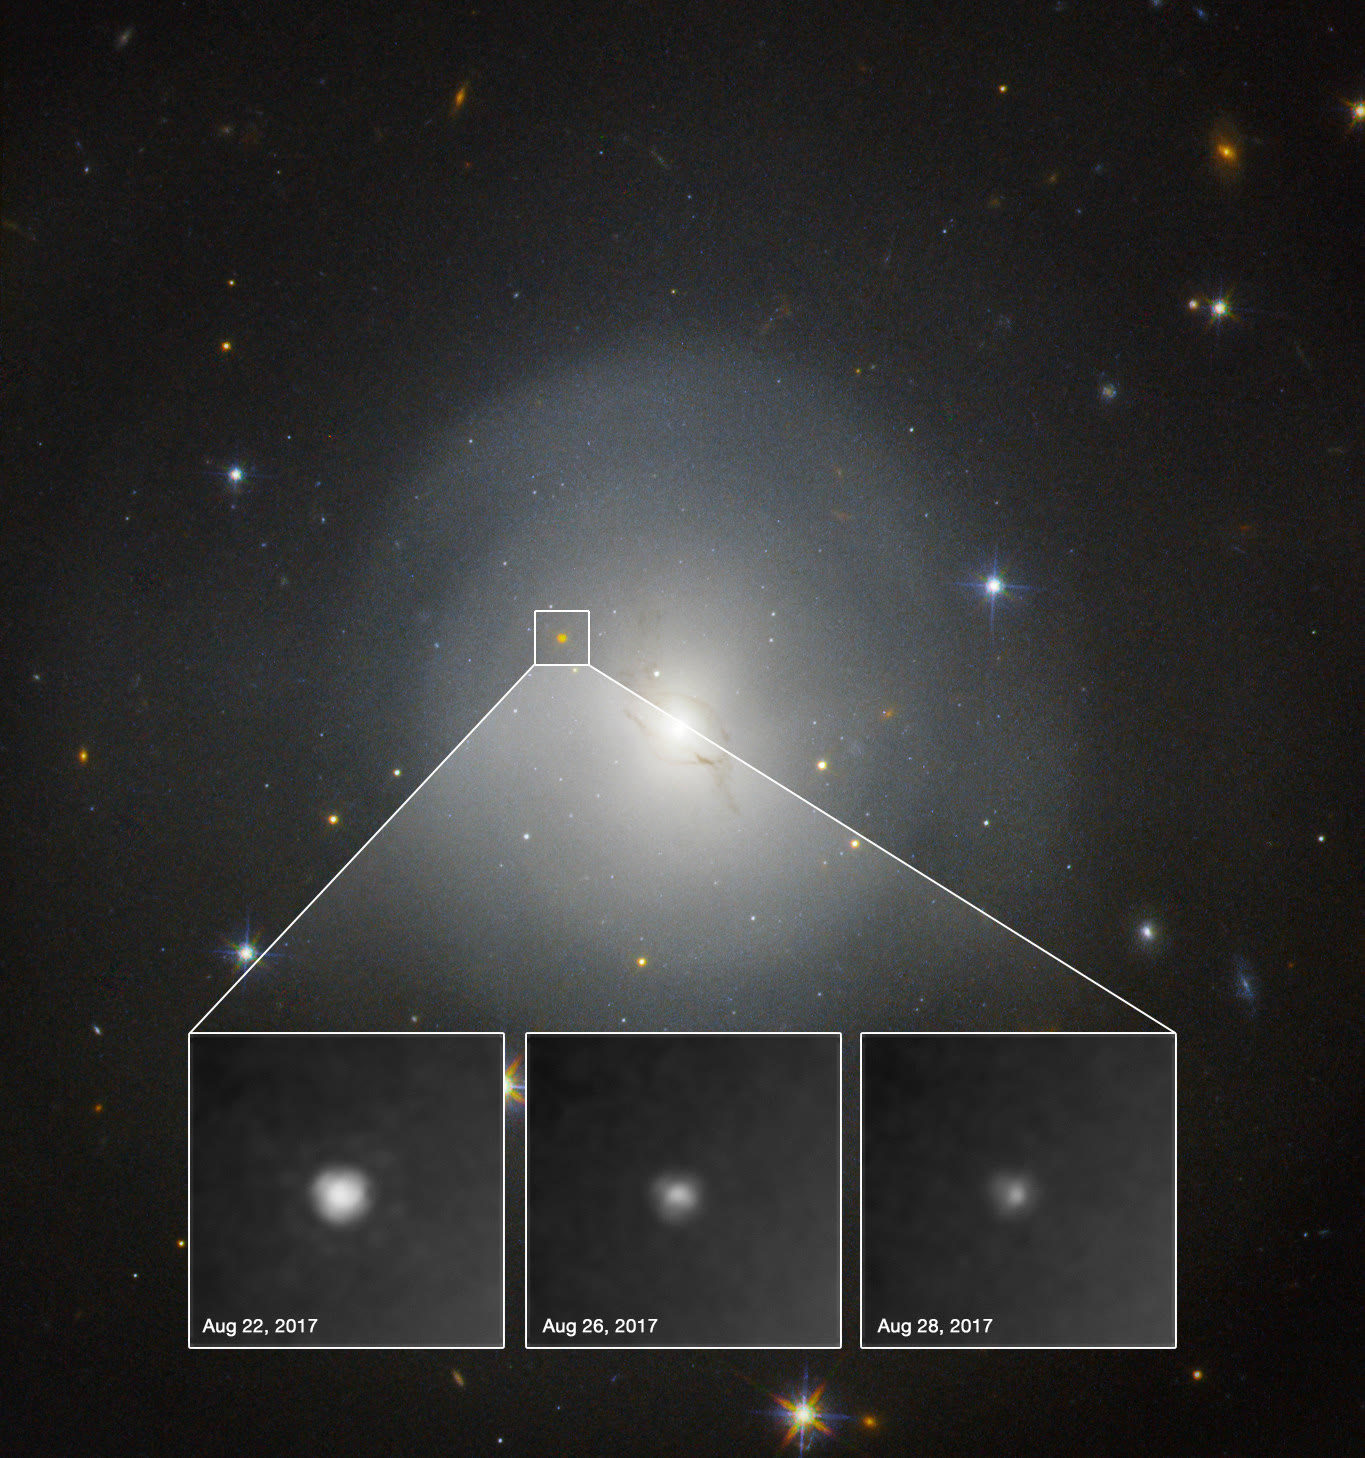
\includegraphics[width=0.55\linewidth]{images/book5/b3-kilonova.jpg}
\par\smallskip{\small Het sterrenstelsel NGC~4993, gefotografeerd door de Hubble
ruimtetelescoop na de samensmelting van twee neutronensterren die in
zwaartekrachtgolven waren waargenomen op 17 augustus 2017. Het vak markeert de \omterm{def:b3:origin-of-elements:kilonova}{kilonova}; de
inzetjes, genomen op 22, 26 en 28 augustus, tonen hoe die in zes dagen verzwakt.
NASA en ESA (A.~J.~Levan, N.~R.~Tanvir, A.~Fruchter en O.~Fox), CC
BY~4.0.}\label{fig:b3:origin-of-elements:kilonova}
\end{omfigure}
% ledger: photo:b3-kilonova

\begin{dated}{2021}
Of samensmeltingen van neutronensterren het grootste deel van de r-proceselementen van de Melkweg maken,
is niet vastgesteld. Samensmeltingen moeten wachten tot hun dubbelsterbanen door uitzending van
zwaartekrachtgolven krimpen, en modellen van de evolutie van de Melkweg waarin zij de enige bron zijn
maken de r-proceselementen te laat om te verklaren wat men ziet in de
oudste, meest metaalarme sterren. Zeldzame soorten kernineenstortingssupernova's,
met snelle rotatie en sterke magneetvelden, en de ineenstorting van zeer zware sterren
zijn de andere kandidaten; één model van de Melkweg verklaart het waargenomen europium
als ongeveer drie procent van de hypernova's van \num{25} tot
\qty{50}{M_\odot} van het magnetisch
aangedreven type zijn.
\end{dated}
% ledger: kobayashi20:origins, cowan21:rprocess

\section{De chemische evolutie van de Melkweg}\label{sec:b3:origin-of-elements:gce}

Elke generatie sterren geeft een deel van wat ze heeft gemaakt terug aan het gas, en
de volgende generatie vormt zich uit dat verrijkte gas. De samenstelling van een
ster legt daarom de samenstelling van het gas op het moment van haar geboorte vast, en de
sterren van een sterrenstelsel, gerangschikt naar ouderdom, leggen zijn geschiedenis vast.

\begin{definition}[Galactische chemische evolutie]\label{def:b3:origin-of-elements:gce}
\emph{galactische chemische evolutie}\index{galactische chemische evolutie}
is de verandering van de samenstelling van het gas en van de sterren van een
sterrenstelsel in de tijd, onder de gecombineerde werking van stervorming, de \omterm{def:b3:origin-of-elements:yield}{stellaire
opbrengsten}, de levensduur van de sterren en het gas dat het sterrenstelsel instroomt of
eruit wordt gedreven; en de bestudering van die verandering met modellen die worden vergeleken
met de abundanties van sterren van bekende ouderdom.
\end{definition}
% ledger: matteucci21:simple

Het eenvoudigste model behandelt een gebied van een sterrenstelsel als één goed gemengde doos
gas dat langzaam in sterren overgaat. Laat $s$ de massa zijn die
is vastgelegd in langlevende sterren en in stellaire overblijfselen, $M_\mathrm{g}$ de massa van
het gas, $M = M_\mathrm{g} + s$ het totaal. De \emph{opbrengst per stellaire
generatie} $y$ is de massa nieuwe metalen die een generatie sterren
per eenheid vastgelegde massa aan het gas teruggeeft.
% ledger: matteucci21:yield

\begin{theorem}[Gesloten-doosmodel]\label{thm:b3:origin-of-elements:closed-box}
\index{gesloten-doosmodel}
Beschouw een gebied dat geen gas uitwisselt met zijn omgeving, dat begint als
zuiver gas zonder metalen, goed gemengd blijft, en waarin de sterren die
metalen maken direct sterven, terwijl de andere eeuwig leven (onmiddellijke
recycling). Dan is de \omterm{def:b3:origin-of-elements:metallicity}{metalliciteit} van het gas
\[
Z = y \ln\frac{1}{\mu}, \qquad \mu = \frac{M_\mathrm{g}}{M},
\]
waarin $\mu$ de gasfractie is, en de massa sterren die zijn gevormd met een
\omterm{def:b3:origin-of-elements:metallicity}{metalliciteit} lager dan $Z$ is \mbox{$M\,(1 - \mathrm{e}^{-Z/y})$}.
\end{theorem}

\begin{proof}
Wanneer een massa $\mathrm{d}s$ in sterren wordt vastgelegd, verliest het gas
$\mathrm{d}s$, samen met de metalen die het bevat, $Z\,\mathrm{d}s$,
en wint $y\,\mathrm{d}s$ aan nieuwe metalen:
$\mathrm{d}M_\mathrm{g} = -\mathrm{d}s$ en
$\mathrm{d}(Z M_\mathrm{g}) = (y - Z)\,\mathrm{d}s$. Uitwerken van de
tweede, $M_\mathrm{g}\,\mathrm{d}Z + Z\,\mathrm{d}M_\mathrm{g} =
y\,\mathrm{d}s - Z\,\mathrm{d}s$, en de termen in $Z$ vallen weg:
$M_\mathrm{g}\,\mathrm{d}Z = -y\,\mathrm{d}M_\mathrm{g}$. Integreren
vanaf $M_\mathrm{g} = M$, $Z = 0$ geeft $Z = y\ln(M/M_\mathrm{g})$. De
sterren die zijn gevormd terwijl de \omterm{def:b3:origin-of-elements:metallicity}{metalliciteit} van het gas lager was dan $Z$ zijn die
gevormd terwijl het gas van $M$ daalde tot $M\mathrm{e}^{-Z/y}$, een massa
$M(1 - \mathrm{e}^{-Z/y})$.
\end{proof}
% ledger: matteucci21:simple

Het model voorspelt de metalliciteitsverdeling van de langlevende sterren.
In de zonnenabuurt bedraagt de oppervlaktedichtheid van het gas
\qty{13.7}{M_\odot.pc^{-2}}, en die van sterren en stellaire overblijfselen
\qty{33.4}{M_\odot.pc^{-2}}, dus $\mu = 13.7/47.1 = 0.29$. Als het gas
vandaag het protosolaire $Z = 0.0154$ heeft, is de opbrengst
$y = 0.0154/\ln(1/0.29) = 0.0125$, en de fractie van alle tot nu toe
gevormde sterren met een $Z$ onder een tiende van de huidige waarde,
$[\mathrm{Fe/H}] < -1$ als ijzer de metalen volgt, is
$(1 - 0.29^{0.1})/(1 - 0.29) = 0.16$.
% ledger: mckee15:surface, asplund21:xyz, data:b5-gce

\begin{omfigure}
\centering
\begin{tikzpicture}
\begin{axis}[width=0.95\linewidth, height=7.2cm, xmin=-1.6, xmax=0.7,
  ymin=0, ymax=1500, xlabel={$[\mathrm{Fe/H}]$},
  ylabel={aantal sterren per \num{0.1}~dex},
  tick label style={font=\scriptsize}, label style={font=\small},
  legend style={font=\scriptsize, at={(0.5,-0.17)}, anchor=north,
    legend columns=3, draw=none, cells={anchor=west},
    /tikz/every even column/.append style={column sep=1em}}]
\addplot[ybar, area legend, bar width=0.085, fill=black!25, draw=black!50, bar shift=0pt]
  table[x=feh, y=n_obs] {figdata/out/bachelor-3-chemical_evolution-mdf.dat};
\addlegendentry{F- en G-dwergen (6670)}
\addplot[ybar, area legend, bar width=0.085, fill=blue!55, draw=blue!70!black, bar shift=0pt]
  table[x=feh, y=n_low] {figdata/out/bachelor-3-chemical_evolution-mdf.dat};
\addlegendentry{hoogstens \qty{1}{M_\odot} (902)}
\addplot[red!75!black, very thick, const plot mark mid]
  table[x=feh, y=model] {figdata/out/bachelor-3-chemical_evolution-mdf.dat};
\addlegendentry{gesloten doos}
\draw[black!50, dashed] (axis cs:-1,0) -- (axis cs:-1,1500);
\node[font=\scriptsize, anchor=north west, align=left] at (axis cs:-1.57,1450)
  {gesloten doos: \qty{16}{\percent}\\onder $-1$;\\waargenomen: \qty{0.4}{\percent}};
\end{axis}
\end{tikzpicture}
\par\smallskip{\small Het \omterm{def:b3:origin-of-elements:g-dwarf}{G-dwergprobleem}. Staven: de \omterm{def:b3:origin-of-elements:metallicity}{metalliciteiten} van
de F- en G-dwergen uit de zonnenabuurt (Geneva--Copenhagen
survey, de steekproef met de beste fotometrie, opnieuw geanalyseerd door Casagrande en anderen,
2011), alle sterren in grijs, die van hoogstens één zonnemassa, de langlevende
sterren die het model telt, in blauw. Lijn: de \omterm{thm:b3:origin-of-elements:closed-box}{gesloten
doos} met de huidige gasfractie van de zonnenabuurt, geschaald naar
hetzelfde aantal sterren; geen ster is rijker dan het huidige gas,
dat geacht wordt de \omterm{def:b3:origin-of-elements:abundance}{zonneabundantie} te hebben. De doos voorspelt een lange staart van metaalarme
sterren die er niet zijn.}\label{fig:b3:origin-of-elements:g-dwarf}
\end{omfigure}
% ledger: data:b5-gcs, casagrande11:gcs, data:b5-gce, mckee15:surface

\begin{definition}[G-dwergprobleem]\label{def:b3:origin-of-elements:g-dwarf}
Het \emph{G-dwergprobleem}\index{G-dwergprobleem} is het tekort aan
metaalarme langlevende sterren in de zonnenabuurt vergeleken met de
voorspelling van het \omterm{thm:b3:origin-of-elements:closed-box}{gesloten-doosmodel}: veel minder van de langlevende dwergsterren
van spectraaltype G hebben lage \omterm{def:b3:origin-of-elements:metallicity}{metalliciteiten} dan een \omterm{thm:b3:origin-of-elements:closed-box}{gesloten doos} zou
hebben opgeleverd.
\end{definition}
% ledger: matteucci21:simple

Van de 6670 sterren van de steekproef hebben er 26 $[\mathrm{Fe/H}] < -1$:
\qty{0.4}{\percent}, tegenover de \qty{16}{\percent} van de \omterm{thm:b3:origin-of-elements:closed-box}{gesloten doos}.
Zelfs onder de 902 sterren van hoogstens één zonnemassa, de eerlijkste
vergelijking zijn de 26 goed voor \qty{2.9}{\percent}. De uitweg is de
doos te openen: als de schijf van de zonnenabuurt is opgebouwd door een langzame
instroom van metaalarm gas gedurende meerdere miljarden jaren, was het vroege gas nooit
een groot reservoir dat wachtte om metaalarme sterren te vormen, en de staart
verdwijnt. Modellen van de schijf die de verdeling reproduceren, hebben een
instroomtijd nodig die langer is dan drie tot vier miljard jaar.
% ledger: data:b5-gcs, data:b5-gce, matteucci21:simple

De tweede klok is de verhouding van twee soorten elementen. De \omterm{def:b3:origin-of-elements:alpha}{alfa-elementen}
komen van kernineenstortingssupernova's, kort nadat een sterrengeneratie
is geboren; veel van het ijzer komt van supernova's van type~Ia,
veel later. In oude halosterren, met $[\mathrm{Fe/H}] < -1$,
$[\alpha/\mathrm{Fe}]$ bedraagt ongeveer $+0.4$: deze sterren zijn gevormd uit gas
dat uitsluitend door kernineenstortingssupernova's was verrijkt. In schijfsterren daalt het met
toenemende \omterm{def:b3:origin-of-elements:metallicity}{metalliciteit} naar nul, de zonnewaarde, omdat de supernova's van type~Ia
hun ijzer toevoegen. De figuur hieronder toont het eenvoudigste model
van dit \emph{vertragingstijd}-beeld: in een \omterm{thm:b3:origin-of-elements:closed-box}{gesloten doos} komen beide soorten
supernova's tegelijk op gang, behalve dat die van type~Ia een vaste
vertraging na de eerste sterren beginnen.
% ledger: matteucci21:time-delay, matteucci21:production

\begin{omfigure}
\centering
\begin{tikzpicture}
\begin{axis}[width=0.8\linewidth, height=6.4cm, xmin=-2.4, xmax=0.25,
  ymin=-0.08, ymax=0.55, xlabel={$[\mathrm{Fe/H}]$},
  ylabel={$[\alpha/\mathrm{Fe}]$},
  tick label style={font=\scriptsize}, label style={font=\small}]
\addplot[black!40, dashed, domain=-2.4:0.25, samples=2] {0};
\addplot[blue!70!black, very thick]
  table[x=feh, y=afe] {figdata/out/bachelor-3-chemical_evolution-alpha.dat};
\addplot[only marks, mark=*, mark size=2pt, red!70!black] coordinates {(-1,0.4) (0,0)};
\node[font=\scriptsize, anchor=south, align=center] at (axis cs:-1.75,0.41)
  {alleen kernineenstortingssupernova's};
\node[font=\scriptsize, anchor=south west, align=left] at (axis cs:-0.98,0.41)
  {supernova's van type Ia\\[-1pt]beginnen};
\node[font=\scriptsize, anchor=south west] at (axis cs:0.01,0.01) {Zon};
\end{axis}
\end{tikzpicture}
\par\smallskip{\small Een tweefasenmodel van $[\alpha/\mathrm{Fe}]$ in een
\omterm{thm:b3:origin-of-elements:closed-box}{gesloten doos}: het plateau op $+0.4$ is de verhouding die door
kernineenstortingssupernova's wordt gemaakt; supernova's van type~Ia, die beginnen wanneer het gas
$[\mathrm{Fe/H}] = -1$ heeft bereikt, voegen dan ijzer toe in een constant tempo, tot de
verhouding zonnewaarde is bij $[\mathrm{Fe/H}] = 0$. Het plateau en de knik zijn die
welke in de sterren van het Melkwegstelsel worden gezien; de vorm daartussen is van het model.
Bij de \omterm{def:b3:origin-of-elements:metallicity}{metalliciteit} van de Zon is \qty{60}{\percent} van het ijzer in dit
model afkomstig van supernova's van type~Ia.}\label{fig:b3:origin-of-elements:alpha}
\end{omfigure}
% ledger: data:b5-gce, matteucci21:time-delay

De gedetailleerde modellen van het Melkwegstelsel die de waargenomen trend
reproduceren, halen tweederde van het ijzer uit supernova's van type~Ia en
eenderde uit kernineenstortingssupernova's, en vinden dat het gas van het jonge
Melkwegstelsel $[\mathrm{Fe/H}] = -1$ bereikte in ongeveer één tot anderhalf
miljard jaar. De verhouding is een klok: een populatie die rijk is aan
\omterm{def:b3:origin-of-elements:alpha}{alfa-elementen} bij een gegeven \omterm{def:b3:origin-of-elements:metallicity}{metalliciteit}, heeft haar sterren snel gevormd, voordat de
supernova's van type~Ia hun ijzer konden toevoegen. De \omterm{def:b3:milky-way-galaxies:structure}{dikke schijf} uit het vorige
hoofdstuk is zo'n populatie: oud, en licht verrijkt met
\omterm{def:b3:origin-of-elements:alpha}{alfa-elementen} vergeleken met sterren uit de dunne schijf bij dezelfde \omterm{def:b3:origin-of-elements:metallicity}{metalliciteit}.
% ledger: matteucci21:time-delay, casagrande11:gcs

\section{Van de zonneabundanties naar de Aarde}\label{sec:b3:origin-of-elements:earth}

De Aarde is opgebouwd uit hetzelfde materiaal als de Zon, maar niet uit al dat
materiaal. In de afkoelende nevel konden alleen de elementen die tot vaste
stoffen condenseerden, konden worden verzameld tot planetesimalen; het boek van jaar~2 volgde de
volgorde waarin ze condenseren. IJzer condenseert als metaal bij ongeveer dezelfde
temperatuur als de magnesiumsilicaten, \qtyrange{1310}{1340}{K} bij
\qty{e-4}{bar}, zodat de rotsplaneten hun aandeel ijzer behielden, terwijl
waterstof, helium, koolstof, stikstof en de edelgassen in het gas bleven.
Van een gas met zonnesamenstelling condenseert slechts ongeveer een half procent
van de massa als gesteente en metaal.
% ledger: lodders:tc-table, lodders:condensates

\begin{definition}[Vluchtigheidstrend]\label{def:b3:origin-of-elements:volatility}
De \emph{vluchtigheidstrend}\index{vluchtigheidstrend} van een planetair lichaam
is de afname van zijn abundanties, ten opzichte van de CI-chondrieten en
genormaliseerd op een refractair element, met afnemende condensatie
temperatuur: refractaire elementen staan in hun chondritische verhoudingen, matig vluchtige
zijn des te meer uitgeput naarmate hun
condensatietemperatuur lager is.
\end{definition}

Voor de silicaataarde tekende het boek van jaar~2 de trend tegen de
condensatietemperatuur. Genormaliseerd op magnesium staat zirkonium
(condenserend bij \qty{1741}{K}) staat op \num{1.11} maal zijn
CI-verhouding, natrium (\qty{958}{K}) op \num{0.22}, kalium
(\qty{1006}{K}) op \num{0.19}, rubidium (\qty{800}{K}) op \num{0.12}
en zink (\qty{726}{K}) op \num{0.075}. De Aarde vormde zich uit materiaal dat
al een deel van zijn matig vluchtige elementen had verloren voordat
de planeet werd samengesteld, of verloor ze tijdens zijn groei. Zelfs de
CI-chondrieten verschillen van de Zon op een manier die de condensatie
temperatuur volgt, zij het zwak: hun matig vluchtige elementen staan
ongeveer \num{0.04}~\omterm{def:b3:origin-of-elements:abundance}{dex} hoger dan de fotosferische waarden.
% ledger: lodders:tc-table, lodders:ci-table, ms95:pm-trace, asplund21:abstract

Het verhaal van dit hoofdstuk loopt dus door de planeet heen. Het zuurstof,
magnesium en silicium van de mantel zijn \omterm{def:b3:origin-of-elements:alpha}{alfa-elementen} van massieve
sterren; het ijzer van de kern kwam grotendeels van supernova's van type~Ia;
het thorium en uranium wier verval helpt het inwendige op te warmen, liggen voorbij
bismut, waar alleen het \omterm{def:b3:origin-of-elements:s-process}{r-proces} komt; en het hele mengsel werd
op vluchtigheid gesorteerd voordat de Aarde het verzamelde.
% ledger: matteucci21:production, matteucci21:time-delay, kaeppeler11:overview, data:b5-sigman

\section{Oefeningen}

\begin{exercise}[$\star$]\label{exo:b3:origin-of-elements:1}
Gebruik de \omterm{def:b3:origin-of-elements:abundance}{zonneabundanties} $\log\varepsilon(\mathrm{O}) = 8.69$,
$\log\varepsilon(\mathrm{Si}) = 7.51$, $\log\varepsilon(\mathrm{Fe}) =
7.46$, $\log\varepsilon(\mathrm{Au}) = 0.91$ en
$\log\varepsilon(\mathrm{Pb}) = 1.95$: (a)~hoeveel siliciumatomen en
hoeveel zuurstofatomen zijn er in de Zon per ijzeratoom? (b)~Hoeveel
ijzeratomen per goudatoom, en hoeveel loodatomen per goudatoom?
\end{exercise}

\begin{exercise}[$\star$]\label{exo:b3:origin-of-elements:2}
(a)~Hoeveel ijzeratomen per miljoen waterstofatomen bevat de Zon
($\log\varepsilon(\mathrm{Fe}) = 7.46$)? (b)~Een halo-ster heeft
$[\mathrm{Fe/H}] = -2$. Hoeveel waterstofatomen bevat hij per ijzeratoom?
(c)~Een andere ster heeft één ijzeratoom op elke tien miljoen
waterstofatomen. Wat is zijn $[\mathrm{Fe/H}]$?
\end{exercise}

\begin{exercise}[$\star$]\label{exo:b3:origin-of-elements:3}
De stabiele isotopen van xenon hebben massagetallen 124, 126, 128, 129, 130,
131, 132, 134 en 136. Onder hun isobaren heeft tellurium ($Z = 52$)
stabiele isotopen 120, 122--126, 128 en 130; jodium ($Z = 53$) alleen 127.
Het s-pad bereikt xenon bij $^{128}\mathrm{Xe}$, via het verval van
$^{128}\mathrm{I}$, en verlaat het bij $^{133}\mathrm{Xe}$, dat vervalt.
Classificeer elke xenonisotoop als alleen s, alleen r, door beide
gevormd, of p-kern.
\end{exercise}

\begin{exercise}[$\star$]\label{exo:b3:origin-of-elements:4}
GW170817 lag op ongeveer \qty{40}{Mpc}, en zijn gammastralen kwamen
\qty{1.7}{s} na de samensmelting aan die in zwaartekrachtgolven werd
waargenomen. (a)~Hoe lang hadden beide signalen gereisd? (b)~Als de
vertraging volledig aan een verschil in de twee snelheden wordt
toegeschreven, hoe groot is dat verschil dan hoogstens als breuk van de lichtsnelheid?
\end{exercise}

\begin{exercise}[$\star\star$]\label{exo:b3:origin-of-elements:5}
De drie alleen-s-isotopen van tellurium hebben protosolaire abundanties
\num{0.1067}, \num{0.0373} en \num{0.1984} per $10^6$ siliciumatomen
($A = 122$, $123$, $124$) en gemiddelde werkzame doorsneden \num{295},
\num{832} en \qty{155}{mb}. (a)~Bereken $\sigma N$ voor elk. (b)~Voorspel
uit $^{122}\mathrm{Te}$ alleen de abundanties van $^{123}\mathrm{Te}$
en $^{124}\mathrm{Te}$, en vergelijk. (c)~Waarom kan de relatie niet
worden toegepast op $^{128}\mathrm{Te}$?
\end{exercise}

\begin{exercise}[$\star\star$]\label{exo:b3:origin-of-elements:6}
In het klassieke model geeft elke kern op het s-pad aan de volgende
een fractie $f = 1/(1 + 1/(\tau_0\langle\sigma\rangle))$ van de
stroom door, met $\tau_0 = \qty{0.306}{mb^{-1}}$. (a)~Bereken $f$ voor
$^{124}\mathrm{Te}$ (\qty{155}{mb}) en voor het neutronenmagische
$^{138}\mathrm{Ba}$ (\qty{4.0}{mb}). (b)~De kernen van
$^{137}\mathrm{Ba}$ tot $^{142}\mathrm{Nd}$ op het pad hebben
werkzame doorsneden \num{76.3}, \num{4.0}, \num{32.4}, \num{11.0},
\num{111.4} en \qty{35.0}{mb}. Met welke factor daalt $\sigma N$ van
$^{136}\mathrm{Ba}$ tot $^{142}\mathrm{Nd}$? (c)~Vergelijk met de
gemeten waarden, \num{27.6} en \qty{7.72}{mb}.
\end{exercise}

\begin{exercise}[$\star\star$]\label{exo:b3:origin-of-elements:7}
Een neutron met thermische energie $kT$ heeft de snelheid
$v_T = \sqrt{2kT/m_\mathrm{n}}$, $m_\mathrm{n} = \qty{1.6749e-27}{kg}$.
(a)~Bereken $v_T$ bij $kT = \qty{8}{keV}$, de temperatuur van de
koolstof-13-laag van een rode reus. (b)~Bereken voor $^{124}\mathrm{Te}$,
met $\langle\sigma\rangle = \qty{155}{mb}$, de gemiddelde tijd tussen
twee invangsten, $1/(n_\mathrm{n}\langle\sigma\rangle v_T)$, voor
$n_\mathrm{n} = 10^6$, $10^8$ en \qty{e10}{cm^{-3}}. (c)~Vergelijk met de
halveringstijden van $^{127}\mathrm{Te}$ (\qty{9.35}{h}) en van
$^{134}\mathrm{Cs}$ (\qty{2.07}{yr}). Welke van de twee is een vertakkingspunt?
\end{exercise}

\begin{exercise}[$\star\star$]\label{exo:b3:origin-of-elements:8}
In de Zon is $\log\varepsilon$ \num{6.30} voor calcium, \num{3.14} voor
scandium en \num{4.97} voor titanium; \num{1.38} voor beryllium,
\num{2.70} voor boor en \num{8.46} voor koolstof. (a)~Hoeveel keer
zeldzamer is scandium dan zijn twee buren? (b)~Hoeveel keer zeldzamer is
beryllium dan koolstof? (c)~Welk kenmerk van de abundantiecurve illustreert
elk, en wat is de oorzaak ervan?
\end{exercise}

\begin{exercise}[$\star\star$]\label{exo:b3:origin-of-elements:9}
In het tweefasenmodel van dit hoofdstuk is het plateau
$[\alpha/\mathrm{Fe}] = P$ de verhouding die door kernineenstortingssupernova's
wordt geproduceerd, en bij $[\mathrm{Fe/H}] = 0$ is de verhouding zonnewaarde. (a)~Toon aan dat het aandeel
van het zonne-ijzer dat door supernova's van type~Ia is gemaakt $1 - 10^{-P}$ is, en
bereken dit voor $P = 0.4$. (b)~Welk plateau zou de twee derde van de
gedetailleerde modellen opleveren? (c)~Een dwergstelsel toont zijn knie
bij $[\mathrm{Fe/H}] = -2$. Wat zegt dat over de stervorming ervan?
\end{exercise}

\begin{exercise}[$\star\star\star$]\label{exo:b3:origin-of-elements:10}
De CI-chondrieten bevatten, in delen per miljoen massa, \num{95870}
magnesium, \num{3.96} zirkonium, \num{5010} natrium, \num{530}
kalium en \num{2.13} rubidium; de silicaataarde bevat
\qty{22.8}{\percent} magnesium en \num{10.5}, \num{2670}, \num{240}
en \num{0.6} delen per miljoen van de overige. Hun 50~procent
condensatietemperaturen zijn \qty{1336}{K} (Mg), \qty{1741}{K} (Zr),
\qty{958}{K} (Na), \qty{1006}{K} (K) en \qty{800}{K} (Rb). (a)~Bereken voor
elk element $(X/\mathrm{Mg})_\mathrm{Aarde}/(X/\mathrm{Mg})_\mathrm{CI}$.
(b)~Zet dit uit tegen de condensatietemperatuur en beschrijf de
trend. (c)~Waarom is magnesium als referentie gekozen?
\end{exercise}

\begin{exercise}[$\star\star\star$]\label{exo:b3:origin-of-elements:11}
Een lekkende doos verliest gas in een wind met een snelheid $\lambda$ keer
zijn stervormingssnelheid, en ontvangt niets. (a)~Toon aan dat voor de \omterm{def:b3:origin-of-elements:metallicity}{metalliciteit} geldt
$Z = \frac{y}{1 + \lambda}\ln\frac{M_\mathrm{g}(0)}{M_\mathrm{g}}$.
(b)~Vergelijk met $y = 0.0125$ de \omterm{def:b3:origin-of-elements:metallicity}{metalliciteit} die bereikt wordt wanneer het gas
tot \qty{29}{\percent} van zijn beginmassa is gevallen, voor $\lambda = 0$ en
$\lambda = 1$. (c)~Waarom zijn kleine sterrenstelsels, met zwakke
zwaartekracht, meestal metaalarm?
\end{exercise}

\begin{exercise}[$\star\star\star$]\label{exo:b3:origin-of-elements:12}
(a)~De Zon heeft $\log\varepsilon(\mathrm{Li}) = 0.96$ in haar fotosfeer
en de CI-chondrieten $3.25$. Bereken de twee verhoudingen $N_\mathrm{Li}/N_\mathrm{H}$
en het aandeel van zijn lithium dat de Zon heeft vernietigd. (b)~De oudste
metaalarme sterren tonen $N_\mathrm{Li}/N_\mathrm{H} = \num{1.45e-10}$,
terwijl de oerknalnucleosynthese \num{4.72e-10} voorspelt. Met welke factor
overtreft het lithium van het Zonnestelsel elk van beide? (c)~Wat impliceren de
twee vergelijkingen?
\end{exercise}

\section{Probleem: Een sterrenstelsel als gesloten doos}

\begin{problem}[{Weekendprobleem --- van het zonnemengsel naar de
metalliciteiten van de langlevende sterren}]
\label{pb:b3:origin-of-elements:1}
Gebruik $\log\varepsilon(\mathrm{H}) = 12$, de \omterm{def:b3:origin-of-elements:abundance}{zonneabundanties}
$\log\varepsilon(\mathrm{Fe}) = 7.46$, $\log\varepsilon(\mathrm{O}) =
8.69$, $\log\varepsilon(\mathrm{He}) = 10.914$, de huidige
fotosferische massafracties $X = 0.7438$, $Y = 0.2423$, $Z = 0.0139$,
en de protozonne $Z_\odot = 0.0154$. Neem overal aan dat ijzer
de totale \omterm{def:b3:origin-of-elements:metallicity}{metalliciteit} volgt, $[\mathrm{Fe/H}] = \log_{10}(Z/Z_\odot)$.

\medskip\noindent\textbf{Deel I --- Het zonnemengsel.}
\begin{enumerate}
\item Hoeveel waterstofatomen zijn er in de Zon per ijzeratoom?
\item Bereken de getalsverhouding $N_\mathrm{He}/N_\mathrm{H}$. Neem een
  heliumatoom dat vier keer zo zwaar is als een waterstofatoom, vergelijk
  $4N_\mathrm{He}/N_\mathrm{H}$ met $Y/X$.
\item Een ster bevat één ijzeratoom op elke \num{350000} waterstofatomen.
  Bereken zijn $[\mathrm{Fe/H}]$ op twee decimalen.
\item Dezelfde ster heeft $[\mathrm{O/Fe}] = +0.40$. Bereken zijn
  $\log\varepsilon(\mathrm{O})$, en het aantal zuurstofatomen per ijzeratoom
  vergeleken met dat van de Zon.
\item Zuurstof is het meest voorkomende metaal. Schat de metaalmassafractie van de ster
  door die van de Zon te schalen met $[\mathrm{O/H}]$.
\item Waarom wordt de \omterm{def:b3:origin-of-elements:metallicity}{metalliciteit} van een ster meestal aan de hand van ijzer gemeten
  in plaats van aan de hand van zuurstof, hoewel zuurstof $Z$ domineert?
\end{enumerate}

\medskip\noindent\textbf{Deel II --- Het s-proces op telluur.} Gebruik
de gegevens uit \cref{exo:b3:origin-of-elements:5}.
\begin{enumerate}[resume]
\item Verklaar aan de hand van de nuklidenkaart waarom $^{122}\mathrm{Te}$,
  $^{123}\mathrm{Te}$ en $^{124}\mathrm{Te}$ uitsluitend door het \omterm{def:b3:origin-of-elements:s-process}{s-proces} worden gevormd.
\item Bereken $\sigma N$ voor de drie isotopen en hun gemiddelde.
\item Voorspel de overvloed van $^{123}\mathrm{Te}$ uit het gemiddelde van de
  andere twee, en geef het verschil met de gemeten waarde in
  procent.
\item $^{128}\mathrm{Te}$ heeft $N = 1.329$ per $10^6$ Si en
  $\langle\sigma\rangle = \qty{44.4}{mb}$. Bereken zijn $\sigma N$ en
  verklaar waarom hij niet op het plateau ligt.
\item Het paar $^{148}\mathrm{Sm}$ en $^{150}\mathrm{Sm}$, dat alleen door het \omterm{def:b3:origin-of-elements:s-process}{s-proces} wordt gevormd, heeft
  $\sigma N = \num{7.43}$ en \qty{8.53}{mb}. Welk aandeel van de stroom
  liep om $^{148}\mathrm{Sm}$ heen, en via welke vertakking?
\item Bij het passeren van $N = 82$ daalt het product van \qty{27.6}{mb}
  ($^{136}\mathrm{Ba}$) naar \qty{7.72}{mb} ($^{142}\mathrm{Nd}$). Welke
  eigenschap van de kernen met $N = 82$ verklaart de daling?
\end{enumerate}

\medskip\noindent\textbf{Deel III --- De gesloten doos.} De zonnenabijheid
heeft \qty{13.7}{M_\odot.pc^{-2}} aan gas en
\qty{33.4}{M_\odot.pc^{-2}} aan sterren en stellaire overblijfselen. Neem aan dat het
huidige gas $Z = Z_\odot$ heeft.
\begin{enumerate}[resume]
\item Bereken de huidige gasfractie $\mu_1$.
\item Bereken de \omterm{def:b3:origin-of-elements:yield}{stellaire opbrengst} per sterrengeneratie $y$ die de \omterm{thm:b3:origin-of-elements:closed-box}{gesloten doos}
  nodig heeft, en de verhouding daarvan tot $Z_\odot$.
\item Bereken $Z$ en $[\mathrm{Fe/H}]$ van het gas wanneer de gasfractie
  was $0.9$, en daarna $0.5$.
\item Bereken de gasfractie op het moment dat het gas
  $[\mathrm{Fe/H}] = -1$ bereikte.
\item Welk deel van de totale massa was toen in sterren vastgelegd?
\item Als de huidige gasfractie in plaats daarvan $0.1$ zou zijn, welke opbrengst
  zou de doos dan nodig hebben?
\end{enumerate}

\medskip\noindent\textbf{Deel IV --- De verdeling van de metalliciteit.}
\begin{enumerate}[resume]
\item Toon aan dat de \omterm{thm:b3:origin-of-elements:closed-box}{gesloten doos} een verdeling van sterren in
  $[\mathrm{Fe/H}]$ oplevert die evenredig is met $Z\,\mathrm{e}^{-Z/y}$, en bepaal de
  $[\mathrm{Fe/H}]$ van de piek.
\item Bereken het aandeel van alle tot nu toe gevormde sterren met
  $[\mathrm{Fe/H}] < -1$.
\item Bereken het aandeel met $[\mathrm{Fe/H}] < -0.5$.
\item In de steekproef van 6670 F- en G-dwergen hebben 26
  $[\mathrm{Fe/H}] < -1$. Hoeveel zou de \omterm{thm:b3:origin-of-elements:closed-box}{gesloten doos} er voorspellen?
\item Onder de 902 sterren van hooguit één zonnemassa worden dezelfde 26
  aangetroffen. Bereken het waargenomen aandeel en verklaar waarom deze deelsteekproef
  de eerlijkere vergelijking is.
\item Bij een huidige gasfractie van $0.1$, hoe groot zou de voorspelde
  fractie onder $-1$ zijn? Lost een andere gasfractie het
  probleem op?
\item Geef het aandeel langlevende sterren met $[\mathrm{Fe/H}] < -1$
  dat de \omterm{thm:b3:origin-of-elements:closed-box}{gesloten doos} voorspelt voor de zonnenabijheid, in procent,
  op twee significante cijfers, en zeg wat de vergelijking met de
  waargenomen sterren impliceert voor de geschiedenis van de schijf.
\end{enumerate}
\end{problem}
% ledger: asplund21:abstract, asplund21:xyz, data:b5-sigman, data:b5-kadonis, mckee15:surface, data:b5-gcs, data:b5-gce, matteucci21:simple
